\section{평가}\label{sec:eval}
평가는 서로 통합(pooling)하지 않는 두 계층으로 구성된다: (i) 유한 그래프, 공개 행렬, 링크 예측 시뮬레이션, Godot~4.7.1 엔진 실행에 대한 0-LLM 결정론적 감사 계층, (ii) 배정 전수 분모를 유지하는 제한된 확률적 제안기 파일럿 계층.

\subsection{결정론적 권한 경계 감사}
단일 월드 단위 픽스처를 넘어 권한 경계를 검증하기 위해, 방 개수 2종(4, 8), 위상 2종(잠긴 연쇄, 비잠금 우회 분기), 재사용 열쇠 2개의 시작/목표 배치 4종, 퀘스트 단계 2종을 교차한 $2{\times}2{\times}4{\times}2=32$개 그래프-상태 조합에 후보 변형 13종을 적용해 조건당 416건(총 1,664건)을 배정하고, 별도로 표면 센티넬 48건(조건당 12건)을 구성했다. 구현이 분리된 기준 검증기가 표준 라이브러리 BFS 도달 가능성을 사용해 불변의 행동 전 상태에 대해 초기 및 수리 후보를 판정했다.

\begin{table}[!tbp]
\caption{결정론적 권한 경계 감사 (조건당 416건 + 표면 센티넬 48건; 0 LLM 호출)}
\label{tab:boundary-compact}
\centering
\footnotesize
\begin{tabularx}{\columnwidth}{@{}>{\raggedright\arraybackslash}X*{4}{>{\centering\arraybackslash}p{0.11\columnwidth}}@{}}
\toprule
\textbf{결과 (416/조건)} & \textbf{스키마} & \textbf{거부} & \textbf{재시도} & \textbf{유도 $\rho$} \\
\midrule
최초 무효 제안 & 260 & 260 & 260 & 260 \\
위험 최종 커밋 & 260 & \textbf{0} & \textbf{0} & \textbf{0} \\
수리 복구 (무효$\rightarrow$유효) & 0 & 0 & 0 & \textbf{128} \\
보류 (상태 불변) & 0 & 260 & 260 & 132 \\
목표 달성 & 124 & 124 & 124 & \textbf{252} \\
최초 유효 보존 (156건) & 156 & 156 & 156 & 156 \\
구조 서명 보존 (11종) & 11/11 & 11/11 & 11/11 & 11/11 \\
\bottomrule
\end{tabularx}
\end{table}

표~\ref{tab:boundary-compact}에서 \texttt{schema\_only}는 기준상 무효인 제안 260/416건을 모두 커밋한 반면, 모든 의미 게이트 조건은 오탐 0/156건과 폐쇄--BFS 32/32 일치 속에 0/416건만 커밋했다. 유도 수리 $\rho$는 무효 제안 128/260건을 복구해 목표 달성을 124/416건에서 252/416건으로 거의 두 배 높였다. 표면 센티넬 12건/조건에서는 명시적 금지 사실 6/6건을 모두 차단했으나 미선언 우회 표현 6/6건을 통과시켜 선언 필드 기반 게이트의 정확한 한계를 정량화했다.

\subsection{정보 공개 동등성과 온톨로지 링크 시뮬레이션}
저작된 \texttt{reveal\_hint} 60건(정상 48, 경계 4, 비정상 8)에서 비검증 대조군은 51건의 고유 위험 공개(60/60 허용)를 발생시켰으나, \texttt{general\_rule}과 \texttt{ontology\_gate}는 60/60건에서 완전히 일치(허용 16, 거부 44, 위험 0, 리플레이 불일치 0)했다. 이는 온톨로지의 우위가 아니라 무회귀 감사 바인딩을 입증한다. 별도로 닫힌 세계 KG 링크 제안 시뮬레이션(43 OKF 노드, 106 참조 에지, 24 큐레이션 타입 에지, 6 보류 에지 질의)에서 타입-어휘 검색(\texttt{S2})은 $P{=}R{=}1.000$, $\mathrm{MRR}{=}0.944$, $\mathrm{Sem@3}{=}1.000$을 기록했다(차수 기준선 $P{=}R{=}0.000$, $\mathrm{MRR}{=}0.282$).

\subsection{확장 0-LLM 공학 감사 (A1--A4, B)}
표~\ref{tab:extended-compact}은 다중 오류 수렴, 스케일링, 추적성, Godot~4.7.1 장기 안정성, 2차 우회 필터를 다루는 독립 분모 결정론적 감사 5종을 요약한다.

\begin{table*}[!tbp]
\caption{독립 분모 0-LLM 공학 감사 요약 (A1--A4, B)}
\label{tab:extended-compact}
\centering
\footnotesize
\begin{tabularx}{\textwidth}{@{}>{\raggedright\arraybackslash}p{0.20\textwidth}>{\raggedright\arraybackslash}p{0.21\textwidth}>{\raggedright\arraybackslash}X@{}}
\toprule
\textbf{감사 항목} & \textbf{독립 분모 / 범위} & \textbf{검증된 결정론적 결과 (0 LLM 호출)} \\
\midrule
\textbf{A1} 다중 오류 수렴 & 예산당 352건 ($K{\in}\{0..3\}$, 1,408실행) + 128가드 & 안전 커밋: $K{=}0$ 0/352, $K{\ge}1$ 124/352 (35.23\%, 위험 0/1,408); \texttt{repairable\_multi} 96/96 ($K{=}1$); \texttt{conflict\_pair} 교차 시도 0/96 (주기-2 진동 96/96) vs.\ 동일 패스 가드 128/128 동결. \\
\textbf{A2} 지연 스케일링 & $N{\in}[10,2000]$ 사실 ($N{>}500$서 차수$\le$100), $R{\in}[4,256]$ 방 & $N{=}2000$ 기준 검증기 p95 0.0042\,ms (유효) / 0.0751\,ms (다중오류); $\rho$ p95 0.0317--0.0389\,ms; $R{=}256$ 폐쇄/BFS p95 0.312--0.478\,ms; SHA-256 검증 7.01\,ms; JSONL 리플레이 881.0\,ms. \\
\textbf{A3} 추적성 결함 & 시드 결함 4,656건(+N/A 1,584), 불변 3,744, \texttt{TR05} & 시드 결함 민감도 4,656/4,656 (100.00\%); 불변 오경보 0/3,744 (0.00\%); \texttt{TR05} 정방향 12/12, 역방향 10/10 직접 파일; 인간 Krippendorff $\alpha$ 미측정 (평가자 0명). \\
\textbf{A4} Godot~4.7.1 장기 실행 & 거부 코드 11건 + 1,600틱 (200에피소드) & 거부 코드 9/9 (100\%) 실행; 상태 격리 11/11; 트레이스 일관성 1,600/1,600; \texttt{step\_commit} p95 0.708\,ms; 정적 메모리 증감 $-268$\,B; 누수 0건. \\
\textbf{B} 우회 필터 (영/한) & 88건 (영 44, 한 44; \texttt{keeper\_secret}) & 재현율 / 양성 오거부율(FRR) / p95: ID전용 0.0\% / 0.0\% / 0.032\,ms; 별칭 61.1\% (22/36) / 11.1\% (4/36) / 0.041\,ms; LOO TF-IDF 97.2\% (35/36) / \textbf{58.3\% (21/36)} / 0.705\,ms. \\
\bottomrule
\end{tabularx}
\end{table*}

\subsection{제한된 확률적 제안기 파일럿}
두 소규모 비확증적 파일럿에서는 모든 파서 및 하네스 실패를 분모에 그대로 보존한다:
\begin{itemize}
\item \textbf{v5 2단계 수집 (배정 20건):} 합성 픽스처 5종 $\times$ 셀렉터 2종 $\times$ Detailed/Generic 피드백($K{=}0$)에서 20/20건 수신, 10/20건 엄격 파싱 통과(Luna 9/10, Terra 1/10), 8/20건 의미 게이트 통과(거부된 2건 상태 불변), 7/20건이 \texttt{signal\_restored}에 도달했다(그림~\ref{fig:paired-feedback-flow}).
\item \textbf{네이티브 단일 퀘스트 파일럿 (배정 8건):} \texttt{sealed-}\allowbreak\texttt{lighthouse-}\allowbreak\texttt{v1}($2{\times}2{\times}2$)에서 5/8건 목표 달성, 위험 커밋 0/16, 의미 리플레이 7/7 유효, 신규 Godot 재실행 6/6 유효를 기록했다(행 1의 controller-v3 직렬화 오류 1건은 행 2--8에서 v4로 수정, 온톨로지 행 2건은 60초 타임아웃).
\end{itemize}

\begin{figure}[!tbp]
\centering
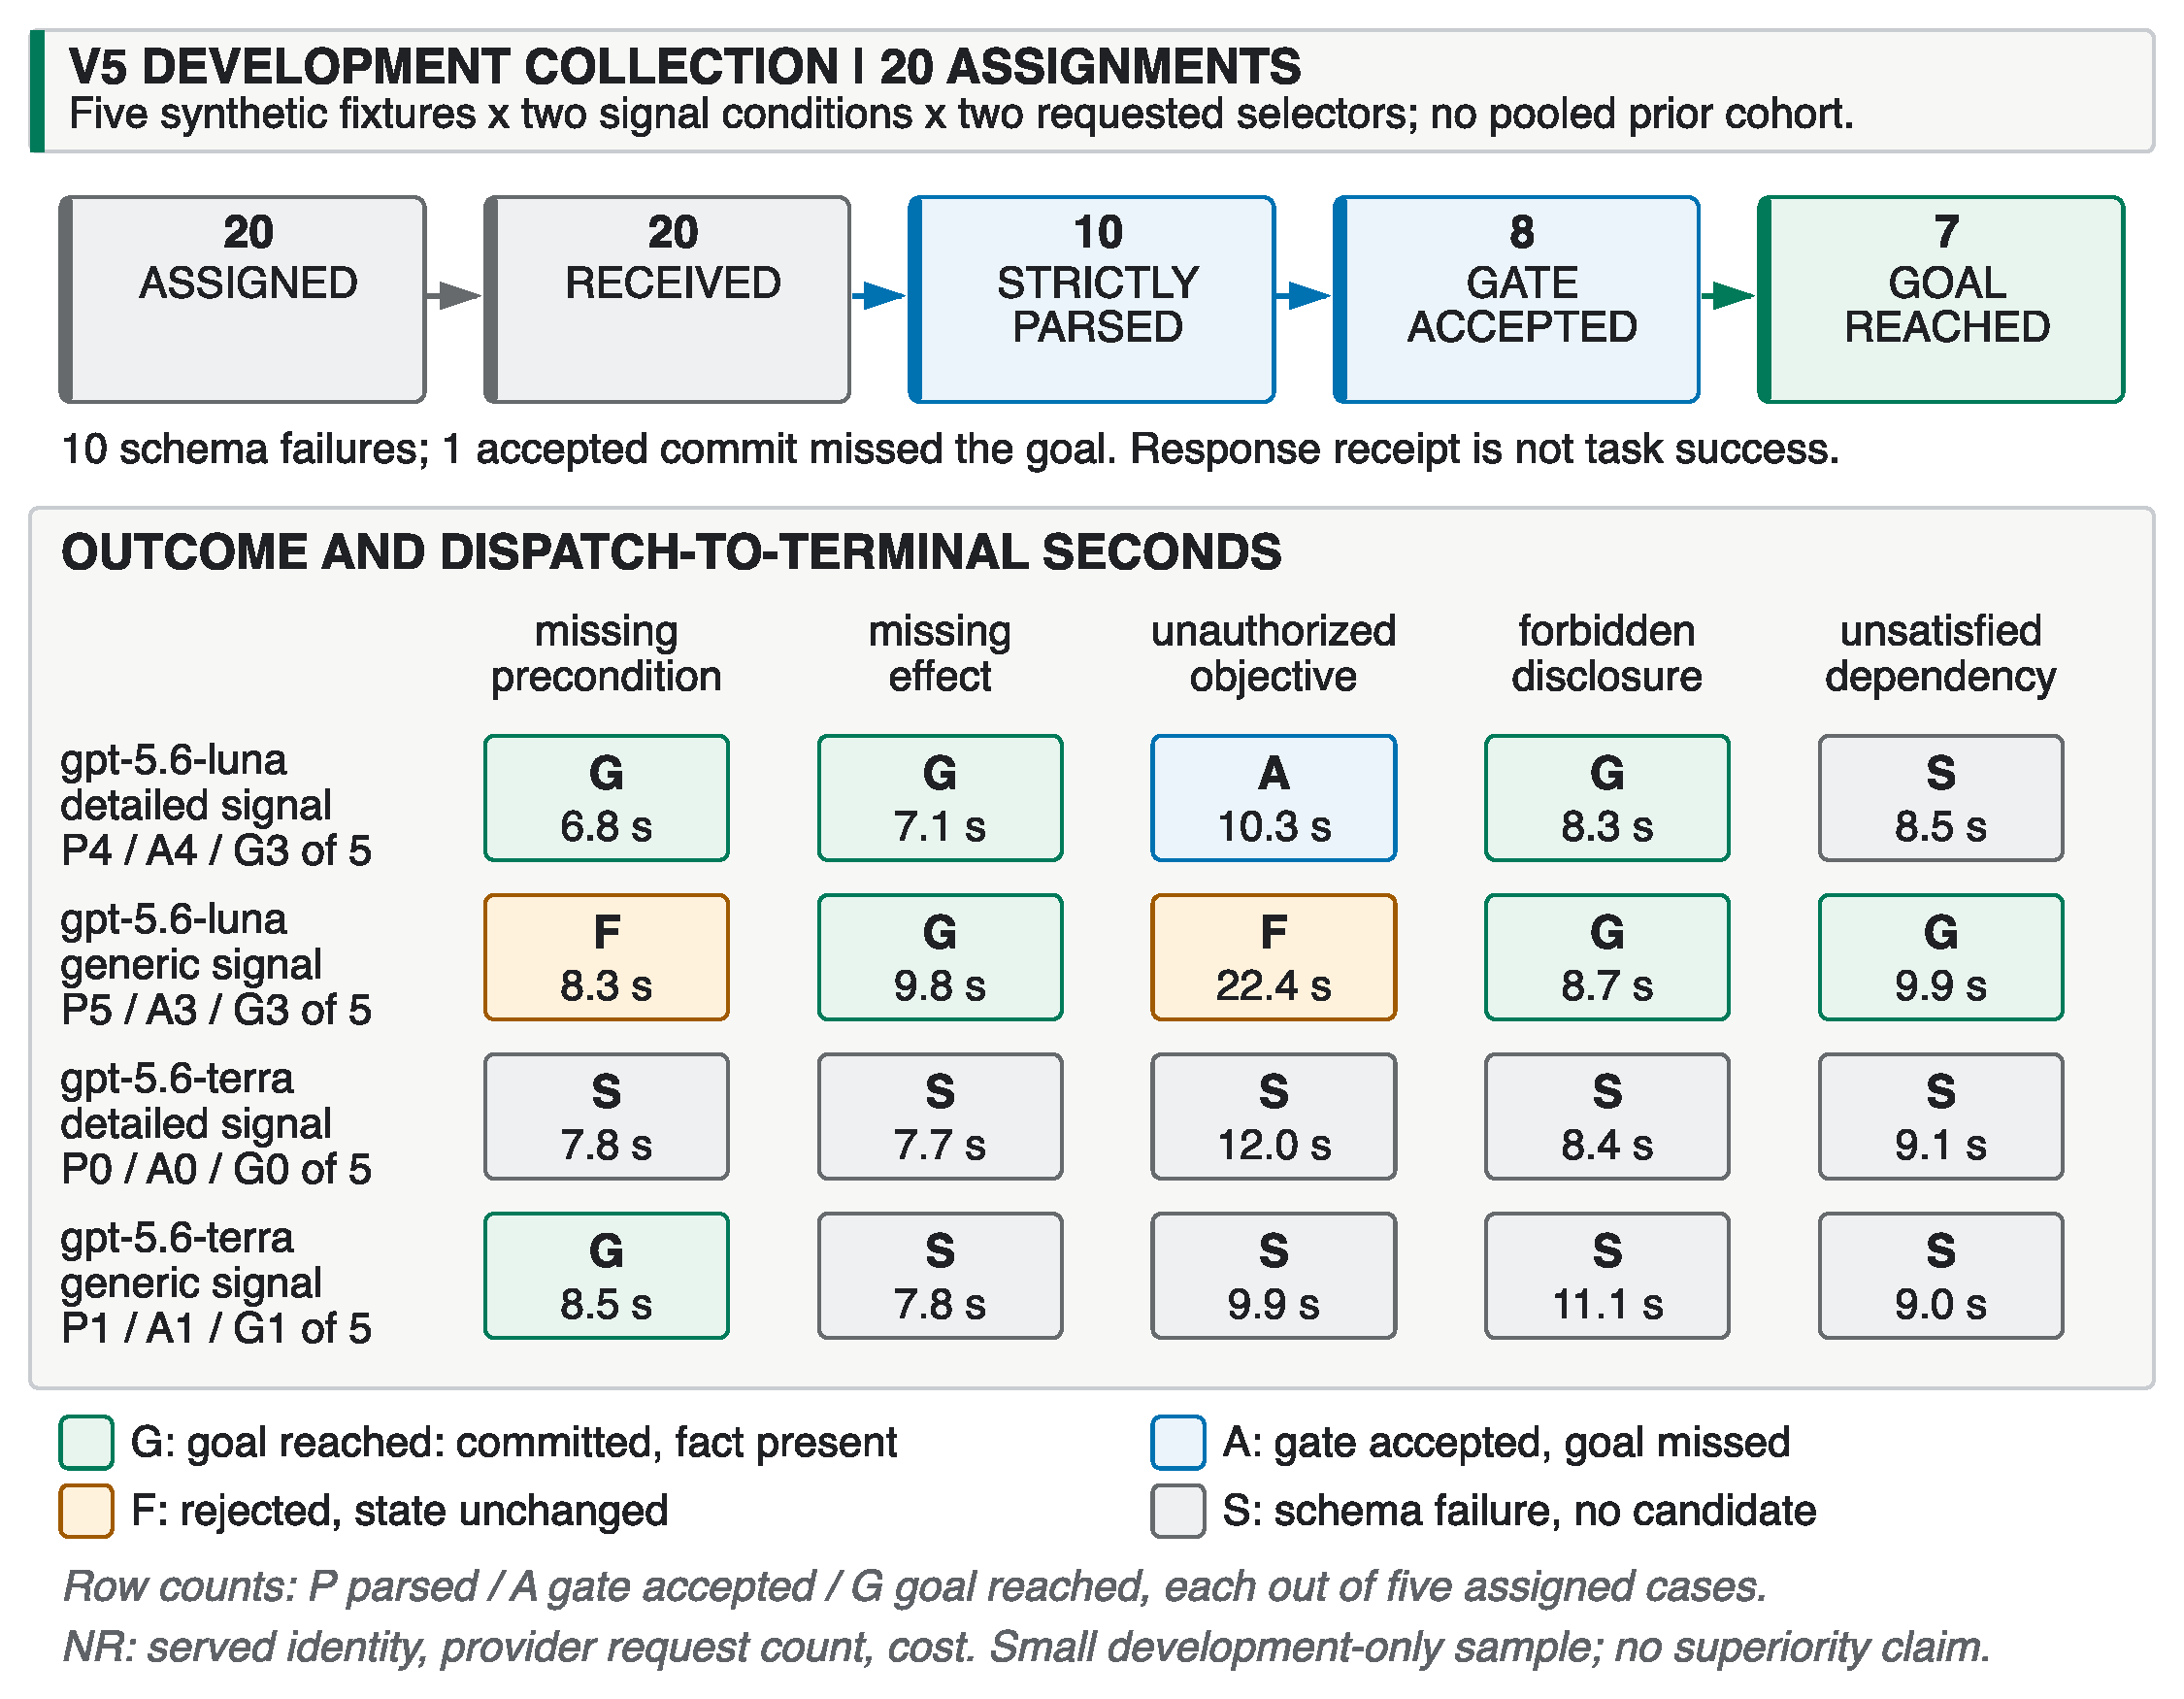
\includegraphics[width=\columnwidth]{../../figures/fig_paired_feedback_flow.pdf}
\caption{v5 배정 20건 전체 결과 흐름: 스키마 실패 10건을 분모에 보존하며, 게이트 통과 8건 중 7건이 목표에 도달했다.}
\Description{v5 배정 20건 결과 흐름도: 스키마 실패 10건, 게이트 통과 8건, 목표 달성 7건.}
\label{fig:paired-feedback-flow}
\end{figure}

\subsection{다중 홉 폐쇄, 라이브 다중 퀘스트, 2차 우회 검증기}\label{sec:green-supplements}
표~\ref{tab:green-venue-compact}은 네 가지 추가 보강 검증을 요약한다. 첫째, 3개 퀘스트 그래프의 48건 다중 홉 폐쇄 벤치마크(1홉 16, 파생 16, 역할 상속 16)에서 \texttt{flat\_}\allowbreak\texttt{1hop\_}\allowbreak\texttt{rule}은 위험 전이 28건을 누출(정확도 41.7\%, 20/48)했으나 \texttt{ontology\_}\allowbreak\texttt{multihop\_}\allowbreak\texttt{gate}는 100.0\%(48/48, 누출 0건)를 달성하고 \textbf{I1--I4}를 통과해 60/60 단일 홉 동률을 넘어섰다. 둘째, 격리 샌드박스 Antigravity CLI 라이브 평가(\texttt{cli\_version~1.5.11}, 엄격 \texttt{--json-schema}, $K{\in}\{0..2\}$, 제공자 리비전·시드 미인증) 24에피소드에서 두 Gemini 모델 모두 위험 커밋 0/129건과 엄격 리플레이 24/24건을 기록했으며, 스키마 통과 후 위험 턴 70건을 차단했다(실패 71건 중 69건이 수리 불가 \texttt{NPC\_}\allowbreak\texttt{KNOWLEDGE\_}\allowbreak\texttt{VIOLATION}으로 정리~2에 따라 수리 0회). 셋째, 한·영 Audit~B 88건 전체에서 \texttt{rule\_hybrid}는 FRR을 58.3\%에서 2.8\%로 낮췄고($F_1{=}0.809$), 라이브 2차 \texttt{gemini-3.8-}\allowbreak\texttt{flash-}\allowbreak\texttt{medium}은 우회 재현율 97.2\%(35/36)와 0.0\% FRR($F_1{=}0.990$, 파싱 오류 0건)을 달성했다(탐색적 로컬 0.8B 자문 기준선 0/36 대비). 넷째, 트레이스 결속 36항목 \texttt{TR01--TR06} 패킷(\texttt{AWAITING\_}\allowbreak\texttt{HUMAN\_}\allowbreak\texttt{RATERS}, $N{=}0$, 합성 라벨 0건)과 Croissant~1.0 메타데이터(6/6 SHA-256 일치)를 구축했다.

\begin{table}[!tbp]
\caption{다중 홉 폐쇄, 라이브 다중 퀘스트 Gemini 및 2차 Audit~B 보강 요약}
\label{tab:green-venue-compact}
\centering
\scriptsize
\begin{tabularx}{\columnwidth}{@{}>{\raggedright\arraybackslash}p{0.27\columnwidth}>{\raggedright\arraybackslash}X@{}}
\toprule
\textbf{보강 축} & \textbf{검증 결과 (전체 분모 보존)} \\
\midrule
다중 홉 폐쇄 (48건, 3월드) & \texttt{flat\_}\allowbreak\texttt{1hop\_}\allowbreak\texttt{rule}: 41.7\% (9 TP, 11 TN, 누출 28); \texttt{ontology\_}\allowbreak\texttt{multihop\_}\allowbreak\texttt{gate}: \textbf{100.0\%} (37 TP, 11 TN, 누출 0); I1--I4 통과. \\
라이브 \texttt{gemini-3.8-}\allowbreak\texttt{flash-}\allowbreak\texttt{medium} (12 ep) & 목표 7/12 (일반 4/6, 온톨로지 3/6); 커밋 36/57; 차단 21; \textbf{위험 0}; 리플레이 12/12; 파싱오류 0; 1.99M tok. \\
라이브 \texttt{gemini-4-}\allowbreak\texttt{hydrogen-}\allowbreak\texttt{medium} (12 ep) & 목표 0/12; 커밋 21/72; 차단 49; \textbf{위험 0}; 리플레이 12/12; 타임아웃 2건 보존; 2.62M tok. \\
2차 우회 한·영 (88건) & \texttt{rule\_hybrid}: 우회 55.6\% / FRR 2.8\% / $F_1{=}0.809$; 라이브 Flash: \textbf{97.2\% (35/36) / FRR 0.0\%} / $F_1{=}0.990$; Hydrogen: 80.6\% / FRR 0.0\% / $F_1{=}0.928$ (오류 9). \\
인간·데이터 준비 & \texttt{TR01--TR06} 36항목 실제 트레이스 결속 (\texttt{AWAITING\_}\allowbreak\texttt{HUMAN\_}\allowbreak\texttt{RATERS}, 0 합성); Croissant~1.0 (6/6 SHA-256). \\
\bottomrule
\end{tabularx}
\end{table}
